%% ****** Start of file template.aps ****** %
%%
%%
%%   This file is part of the APS files in the REVTeX 4 distribution.
%%   Version 4.0 of REVTeX, August 2001
%%
%%
%%   Copyright (c) 2001 The American Physical Society.
%%
%%   See the REVTeX 4 README file for restrictions and more information.
%%
%
% This is a template for producing manuscripts for use with REVTEX 4.0
% Copy this file to another name and then work on that file.
% That way, you always have this original template file to use.
%
% Group addresses by affiliation; use superscriptaddress for long
% author lists, or if there are many overlapping affiliations.
% For Phys. Rev. appearance, change preprint to twocolumn.
% Choose pra, prb, prc, prd, pre, prl, prstab, or rmp for journal
%  Add 'draft' option to mark overfull boxes with black boxes
%  Add 'showpacs' option to make PACS codes appear
%  Add 'showkeys' option to make keywords appear
\documentclass[aps,prl,preprint,groupedaddress]{revtex4}
%\documentclass[aps,prl,preprint,superscriptaddress]{revtex4}
%\documentclass[aps,prl,twocolumn,groupedaddress]{revtex4}
\usepackage{graphicx}
\usepackage{mathtools}
\usepackage{fancyref}
\usepackage[utf8]{inputenc}

% You should use BibTeX and apsrev.bst for references
% Choosing a journal automatically selects the correct APS
% BibTeX style file (bst file), so only uncomment the line
% below if necessary.
%\bibliographystyle{apsrev}

\begin{document}

% Use the \preprint command to place your local institutional report
% number in the upper righthand corner of the title page in preprint mode.
% Multiple \preprint commands are allowed.
% Use the 'preprintnumbers' class option to override journal defaults
% to display numbers if necessary
%\preprint{}

%Title of paper
\title{Towards Entropic Trapping of DNA in Solid-State Nanopores}

% repeat the \author .. \affiliation  etc. as needed
% \email, \thanks, \homepage, \altaffiliation all apply to the current
% author. Explanatory text should go in the []'s, actual e-mail
% address or url should go in the {}'s for \email and \homepage.
% Please use the appropriate macro foreach each type of information

% \affiliation command applies to all authors since the last
% \affiliation command. The \affiliation command should follow the
% other information
% \affiliation can be followed by \email, \homepage, \thanks as well.
\author{Lucas Eggers}
%\email[]{Your e-mail address}
%\homepage[]{Your web page}
%\thanks{}
%\altaffiliation{}
\affiliation{Brown University}

%Collaboration name if desired (requires use of superscriptaddress
%option in \documentclass). \noaffiliation is required (may also be
%used with the \author command).
%\collaboration can be followed by \email, \homepage, \thanks as well.
%\collaboration{}
%\noaffiliation

\date{\today}

\begin{abstract}
% insert abstract here
\end{abstract}

% insert suggested PACS numbers in braces on next line
\pacs{}
% insert suggested keywords - APS authors don't need to do this
%\keywords{}

%\maketitle must follow title, authors, abstract, \pacs, and \keywords
\maketitle

% body of paper here - Use proper section commands
% References should be done using the \cite, \ref, and \label commands
\section{Introduction}

Better nanofluidic control over DNA will yield exciting leaps in technology, such as biochemical labs-on-a-chip and so-called DNA hard drives. We intend to get a few steps closer by making an isolation chamber to hold single DNA molecule in place. Such an isolation chamber would allow for the outcome of biochemical experiments to be observed on a per-molecule basis. It could also act as a storage medium for data encoded in DNA which can hold the equivalent of one million CDs in a single gram for 10,000 years\cite{dna-hard-drive}. We believe we can create such an isolation chamber based on entropic trapping, and combine it with a molecular detector called a nanopore.

In order to isolate a single DNA molecule in the chamber, we need a way to deliver it and to know when it enters. Nanopores are the ideal device for such purposes. A nanopore is a small hole in a membrane, be it biological or synthetic. Solid-state nanopores consist of a hole approximately 10 nanometers across in some larger solid-state membrane. For contrast, double-helical DNA is approximately 2.5 nanometers across. When placed between two reservoirs of ionic solution, solid-state nanopores can detect the passage of a single DNA molecule. This passage event is also known as a translocation. When a voltage bias is placed across the two reservoirs, current forms from ions flowing through the pore. DNA, driven by electrophoretic forces on its slight negative charge, travels toward the pore, eventually getting sucked through. Its passage displaces some flowing ions, causing an observable drop in the ionic current through the pore.

In order to trap DNA in its isolation chamber, we intend to take advantage of the DNA’s configurational entropy. At equilibrium, DNA forms a random coil whose spherical shape has a size characterized by the radius of gyration (Rg). If we could get DNA in a cavity that is roughly the size of the radius of gyration and that has holes smaller than the radius of gyration on either side, we predict that the molecule will have a near-zero probability of diffusing out (Del Bonis-O’Donnel); it would have to squeeze too far out of equilibrium to exit this entropic trap.

\begin{figure}
\centering
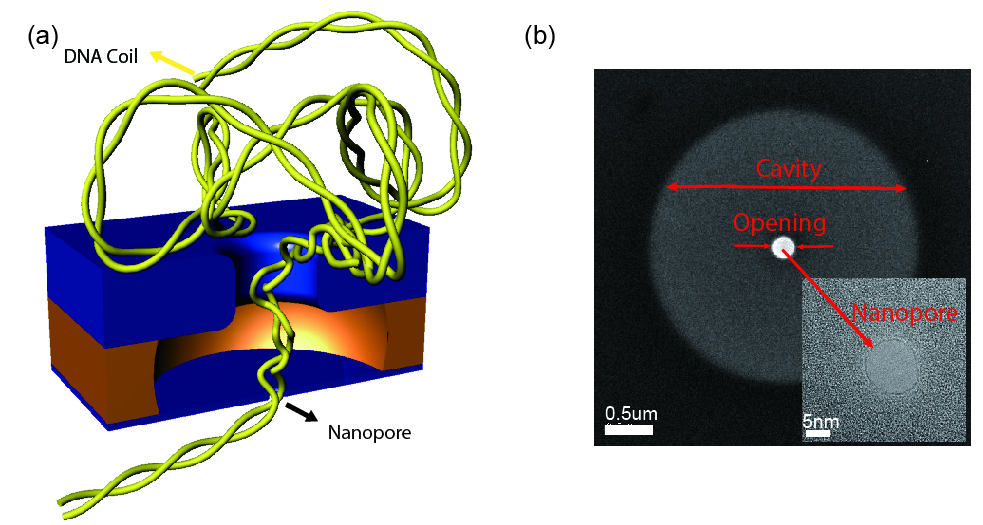
\includegraphics[width=.4\textwidth]{figures/nanopore-schematic}
\caption{A schematic of a silicon structure containing a nanopore and adjacent chamber during a DNA translocation event. The structure has 3 main layers. From bottom to top they are the nanopore, the cavity, and a large hole with diameter approximately 500 nm on average.}
\label{fig:nanopore-schematic}
\end{figure}

The device we envisioned to trap individual DNA molecules is shown in Fig.~\ref{fig:nanopore-schematic}. (Note that the molecule pictured is not trapped.) Capturing a DNA molecule in the cavity can be thought of as a competition between two timescales: the time required to push the center of mass of the DNA through the structure and the time it takes the DNA molecule to equilibrate in the cavity so it cannot traverse the large hole. A translocation starts when the leading tip of DNA  - or someplace nearby on the polymer - enters the nanopore. A drop in current is observed. The molecule is driven through the cavity by local electric fields. As it is driven, Brownian motion causes the molecule to start to equilibrate and expand to fill the chamber. However, translocation happens much faster than equilibration, so the molecule remains ``skinny'' when compared to the large hole; continuing to push it will cause it to exit the structure. Thus, the probability of exit is dependent on the cavity length and hole diameter. When the molecule finishes translocating the current will return to its original baseline value. Turning off the driving voltage at the right moment (too ambiguous? i feel like we could turn off voltage a little before translocation ends if we could calculate it on the fly) will allow the molecule to equilibrate inside the cavity, trapping it.

Placing such a structure between two reservoirs of ionic solution yields the translocation dynamics described above with a twist: the structure’s asymmetry means translocations from either side of the pore are not equivalent. Although the effects of the asymmetric structure on translocation dynamics will be touched on, Karri DiPetrillo's thesis takes a deeper look at those phenomena. The focus of this thesis will be trapping DNA molecules approaching the exposed nanopore (the bottom layer in Fig.~\ref{fig:nanopore-schematic}). Our objectives are thus twofold: to develop the hardware (pores-plus-chambers) and the software (control electronics and data analysis) to make our vision a reality. My contributions were software for analysis and recommendations for programming control electronics informed by my preliminary experiments and theoretical calculation. In addition to creating more intricate labs-on-a-chip and possibly storing DNA hard drives, creating such entropic traps would yield deeper understanding of DNA as a polymer more generally. 
% Put \label in argument of \section for cross-referencing
%\section{\label{}}
\section{Theory}

\subsection{Quantifying DNA as a Polymer}

To know how to trap a DNA molecule, we must understand the constraining length- and timescales. To find the lengthscales we use statistical models of polymers and to find timescales we use a model of polymer dynamics that agrees with the statistical models. We use \(\lambda\)-DNA in our experiments.

The simplest statistical model of a polymer in equilibrium has two parameters: total length \(L\) and persistence length \(p \ll L\). These two numbers describe a freely-jointed chain of length \(L\) in which rigid lengths of polymer of size \(p\) are connected by joints that can take any bond angle. The resulting shape of such an object is a sphere. Mathematically the chain can be described by a three-dimensional random walk. As such, one would expect the radius of the sphere, also known as the radius of gyration, to scale with the square root of the length of the chain: \(R_g \propto L^{1/2}\). The flaw in such reasoning is that real polymers are self-avoiding, meaning that links in the chain cannot occupy the same space. The Flory model modifies the random walk by using a mean field approach (where segments encounter one another with equal probability) to define a new parameter, the Flory exponent \(\nu_F\), where \(R_g \propto L^{\nu_F}\). The Flory model predicts that, for DNA, \(\nu_F = \frac{3}{5}\). Experiments yield an exponent of approximately .588. To make the Flory model even more realistic, we must take into account Brownian motion. The Rouse model describes a polymer as a collection of beads connected by springs in which beads feel the effects of thermal forces and drags. It does not, however, take into account self-avoidance and as such is as useless as the Flory model. 

Timescales are provided by the Zimm model. Zimm combined the Flory and Rouse models by including the hydrodynamic interactions between different parts of the chain as mediated by the solvent. The Zimm model's predictions most exactly agree with experiment. The Zimm model predicts that a polymer enters its equilibrium state from any other state within a characteristic relaxation time \(\tau_z\). That is, if one stretched a DNA molecule to be completely straight, it would reach a spherical conformation in \(\tau_z\) seconds, maximum. The process of reaching such a sphere is known as relaxation. For \(\lambda\)-DNA \(\tau_z \approx 100\)ms. Our translocations last \(\approx 2\)ms, so molecules do not have time to equilibrate until long after they translate. Thus our translocations are called ``fast translocations.'' To paint a physical picture of what that means, we imagine a randomly coiled rope being pulled off a table. As it is pulled, individual folds are sequentially straightened and pulled off the table. Only a small length of rope (the most recently straightened fold) is involved in the motion. The rest of the rope is stationary. The same things happens with DNA, but on a much smaller length scale (put in how many orders of magnitude here, for kicks). Folds of the molecule are sequentially straightened as they are sucked through the pore while the rest of the molecule is effectively frozen.

\subsection{Trapping in More Detail}

Trapping can be thought of as a competition between the movement of DNA through the pore-plus-cavity structure and the equilibration of the molecule in the cavity. The major force pushing the DNA molecule though the structure is electrophoretic. From charge conservation we know that, to a good approximation, the current traveling through the pore (our measured quantity) is equal to the current passing through the area of hemisphere enclosing the pore: 
\begin{equation} I = 2 \pi R^2 J(R) \label{eq:constant-current}\end{equation} 
where \(I\) is current, \(R\) is distance from pore, and \(J(R)\) is the current density. Solving Eq.~\ref{eq:constant-current} for \(J(R)\) we see 
\[J(R) = \frac{I}{2 \pi R^2}.\] 
By Ohm's Law we know 
\[\overrightarrow{J}(R) \equiv \sigma \overrightarrow{E}(R),\]
where \(\sigma\) is two-dimensional charge density.
Combining these equations and solving for E yields:
\begin{equation} E(R) = \frac{I}{\sigma 2 \pi R^2} \label{eq:electric-field} \end{equation} 
We know the velocity of the DNA molecule a distance \(R\) from the pore: 
\begin{equation} v_{\mathrm{DNA}} = \mu_{\mathrm{DNA}} E(R) \label{eq:velocity} .\end{equation} 
Plugging in Eq.~\ref{eq:electric-field} we see that
\[v_{\mathrm{DNA}} = \frac{\mathrm{d}R}{\mathrm{d}t} = \mu_{\mathrm{DNA}} \frac{I}{\sigma 2 \pi R^2},\]
where \(\mu_{DNA}\) is the electrophoretic mobility of DNA.
Integrating yields the tip's distance from the pore and the elapsed time:
\[\int_{R=0}^{R(\Delta t)} \frac{\sigma 2 \pi R^2}{\mu_{\mathrm{DNA}} I} \mathrm{d}R = \int_{t=0}^{\Delta t} \mathrm{d}t \]
yields an equation
\[\frac{1}{3} \frac{\sigma 2 \pi R^3}{\mu_{DNA} I} = \Delta t,\]
which can be solved for \(R(\Delta t)\):
\begin{equation} R(\Delta t) = \sqrt[3]{\frac{3 \mu_{DNA} I}{\sigma 2 \pi}\Delta t} .\label{eq:competition}\end{equation}
Eq.~\ref{eq:competition} quantifies the location of the tip as a function of time. If \(R(\Delta t)\) is less than the height of the cavity, the molecule should be trapped. Even if the tip could travel outside of the chamber (that is, \(R(\Delta t)\) greater than cavity height), we believe the molecule will still be trapped with high probability if the center of mass is within the cavity. The center of mass, the point from which \(R_g\) is measured, should be at approximately \(R(\Delta t)/2\). Plugging in some values from our experiments, \(\mu_{DNA} = 3.75 \times 10^{-3}\)cm$^2$/V$\cdot$s, \( = 3.75 \times 10^{-7}\)m$^2$/V$\cdot$s \cite{mobility} \(I = 20 \mathrm{nA} = 2\times 10^{-8}\mathrm{A}, \Delta t = 2\mathrm{ms} = \mathrm{ms} = 2 \times 10^{-3}\)s and \(\sigma = 850\mu\)S \(= 8.5\times 10^{-4}\)S\cite{conductivity}, we see that the molecule travels \[R(\Delta t) = \sqrt[3]{\frac{3 \mu_{DNA} I}{\sigma 2 \pi}\Delta t} = \sqrt[3]{\frac{3\cdot 3.75\times 10^{-7}\cdot 2\times10^{-8}}{8.5\times10^{-4}\cdot 2\cdot \pi} 2\times10^{-3}}\] \[\approx 2.03 \times 10^{-5}\mathrm{m} = 2.03 \times 10^4 \mathrm{nm} \] in the time it takes to translocate. (half of?) This gives us a lower bound for cavity length. Because our cavities were roughly \(2000\)nm long and we did not kill the voltage immediately after translocation, we captured no DNA molecules in our preliminary trials. We now understand why and are seeking to fabricate devices with longer chambers and build and program better control electronics to improve responsiveness. 

\section{Experiment}

\subsection{Synthesis of Nanopores}



\subsection{DNA Preparation and Apparatus Setup}



\subsection{Trapping Procedure}



\subsection{Data Analysis with MatLab}



\subsubsection{Monodirectional Translocations}



\subsubsection{``Ping-Pong'' Translocations}



\section{Results and Discussion}



\section{Conclusion}


% If in two-column mode, this environment will change to single-column
% format so that long equations can be displayed. Use
% sparingly.
%\begin{widetext}
% put long equation here
%\end{widetext}

% figures should be put into the text as floats.
% Use the graphics or graphicx packages (distributed with LaTeX2e)
% and the \includegraphics macro defined in those packages.
% See the LaTeX Graphics Companion by Michel Goosens, Sebastian Rahtz,
% and Frank Mittelbach for instance.
%
% Here is an example of the general form of a figure:
% Fill in the caption in the braces of the \caption{} command. Put the label
% that you will use with \ref{} command in the braces of the \label{} command.
% Use the figure* environment if the figure should span across the
% entire page. There is no need to do explicit centering.

% \begin{figure}
% \includegraphics{}%
% \caption{\label{}}
% \end{figure}

% Surround figure environment with turnpage environment for landscape
% figure
% \begin{turnpage}
% \begin{figure}
% \includegraphics{}%
% \caption{\label{}}
% \end{figure}
% \end{turnpage}

% tables should appear as floats within the text
%
% Here is an example of the general form of a table:
% Fill in the caption in the braces of the \caption{} command. Put the label
% that you will use with \ref{} command in the braces of the \label{} command.
% Insert the column specifiers (l, r, c, d, etc.) in the empty braces of the
% \begin{tabular}{} command.
% The ruledtabular enviroment adds doubled rules to table and sets a
% reasonable default table settings.
% Use the table* environment to get a full-width table in two-column
% Add \usepackage{longtable} and the longtable (or longtable*}
% environment for nicely formatted long tables. Or use the the [H]
% placement option to break a long table (with less control than 
% in longtable).
% \begin{table}%[H] add [H] placement to break table across pages
% \caption{\label{}}
% \begin{ruledtabular}
% \begin{tabular}{}
% Lines of table here ending with \\
% \end{tabular}
% \end{ruledtabular}
% \end{table}

% Surround table environment with turnpage environment for landscape
% table
% \begin{turnpage}
% \begin{table}
% \caption{\label{}}
% \begin{ruledtabular}
% \begin{tabular}{}
% \end{tabular}
% \end{ruledtabular}
% \end{table}
% \end{turnpage}

% Specify following sections are appendices. Use \appendix* if there
% only one appendix.
%\appendix
%\section{}

% If you have acknowledgments, this puts in the proper section head.
\begin{acknowledgments}
% put your acknowledgments here.
\end{acknowledgments}

% Create the reference section using BibTeX:
\bibliography{bibliogrpahy}

\end{document}
%
% ****** End of file template.aps ******
